% This is samplepaper.tex, a sample chapter demonstrating the
% LLNCS macro package for Springer Computer Science proceedings;
% Version 2.20 of 2017/10/04
%
\documentclass[runningheads]{llncs}
%
\usepackage{graphicx}
% Used for displaying a sample figure. If possible, figure files should
% be included in EPS format.
%
% If you use the hyperref package, please uncomment the following line
% to display URLs in blue roman font according to Springer's eBook style:
% \renewcommand\UrlFont{\color{blue}\rmfamily}

\begin{document}
\bibliographystyle{plainurl}

%
\title{Compiling Files in Parallel: A Study with GCC\thanks{Supported by organization x.}}
%
%\titlerunning{Abbreviated paper title}
% If the paper title is too long for the running head, you can set
% an abbreviated paper title here
%
\author{Giuliano Belinassi\inst{1} \and Richard Biener\inst{2} \and
Alfredo Goldman\inst{1}}
%
\authorrunning{F. Author et al.}
% First names are abbreviated in the running head.
% If there are more than two authors, 'et al.' is used.
%
\institute{Institute of Mathematics and Statistics, São Paulo SP, BRA\\
\url{https://www.ime.usp.br} \and
SuSE Labs, Nürnberg 90409, GER\\
\url{https://www.suse.com/}}

%
\maketitle              % typeset the header of the contribution
%
\begin{abstract}

Processors are becoming increasingly parallel over time, but compiling
software has so far been a task parallelizable only by the number of
files in it. To improve compilation parallelism granularity, we propose
a method feasible to implement in commercial compilers for single file
parallel compilation, with simple modifications in the Link Time
Optimization (LTO) engine in compilers; which we show by implementing
it in GCC. This method resulted in a 20\% speedup when self-compiling
GCC in this mode, and we found no meaningful slowdown when compiling
other applications. We also briefly discuss how this impacts the
Reproducible Builds project.

\keywords{Compilers \and Parallel Compilation \and Link Time Optimization \and LTO.}
\end{abstract}
%
%
%
\section{Introduction}

The recent advances in both technological and computational fields induced an
increasingly faster expansion of software ecosystems. Developers create new
programs to supply the needs of the most diverse domains, either through web
systems coded in script languages; or by components to an operating system
destined to control some hardware resources. Independently of the reason behind
the development of such systems, it is true that their code will be, in some
point, transformed into machine language by a compiler or assembler, even if it
is executed by an interpreter.

Compilers are enormous programs, largely adopted by industry and academy, where
a great effort was and still is employed so that they produce efficient code --
but without any sacrifice in correctness --. There are huge projects destined
to develop and improve them, such as the GNU Compiler Collections
(GCC\footnote{https://gcc.gnu.org/}) and LLVM\footnote{https://llvm.org/}, capable
of translate several languages such as C, C++, and Fortran, to machine language.

GCC was started by Richard Stallman, with the first public release in March of
1987. Back then, it
only supported C language, but already allowed code generation for several
architectures \cite{gcc-first-ver}. Initially designed to compile programs a
single file at time, it could not allow global cross-file optimizations because
the compiler never had the opportunity to analyze the program as a whole. This
changed when Link Time Optimization (LTO) was proposed \cite{whoprgoogle} and
implemented in GCC \cite{glek2010optimizing}. LTO can be enabled in GCC by
using \texttt{-flto}.

In this paper we will present (1) the previous efforts in compile a single
file in parallel, (2) an introduction to how LTO works in GCC, (3) our
proposed changes to LTO for single-file compilation, (4) Results, and
future works and how to improve from here.

\section{Related Works}

Parallel compilation have two main branches, the first being \textit{Parallel
Parsing} and the second being \textit{Parallel Analysis}. Given an alphabet
$\mathrm{\Sigma}$, parsing can be described as building a machine to decide if
an input string $w \in \mathrm{\Sigma}^*$ is a member of a certain language $L
\subseteq \mathrm{\Sigma}^*$ or not, creating the Abstract Syntax Tree in the
process by logging the used derivation rules.  Parallel Compilation includes
parsing (parallel or not), but also includes how to perform analysis,
optimization, and code translation in parallel.

Parallel Parsing dates back from the 1970. \cite{Lincoln:1970:PPT:987475.987478}
explored how to use the vectorial registers in the (so far)
STAR-100 supercomputer for lexical analysis.
\cite{fischer1975parsing} give a detailed theoretical study, proving
several concurrent parsing techniques for LR($k$), LALR($k$) and SLR($k$).
It proceeds by breaking the input in several arbitrary parts, and running a
serial parser on each of these parts. Then the algorithm tries to
recover the stack of each noninitial parser by constructing a set of
possible states, for which there are 5 possible cases. However, in case
of an error, the parser result should be discarded, and therefore a lot
of work will be done in vain when comparing with the sequential version.

But perhaps the most interesting work is by
\cite{Barenghi:2015:PPM:2839536.2840146}, where they explore properties of
Operator Precedence Grammars to construct an Yacc-like parser constructor named
PAPAGENO, which generates parallel parsers. The authors managed to describe a
grammar for Lua and JSON parsing, which they used in their tests. The authors
managed a speedup of up to $5.5\times$ when compared to a parser generated by
GNU Bison.

As for parallel compilation \textit{de facto}, there are two relevant works by
\cite{vandevoorde1988parallel} for C , and \cite{wortman1992} for Modula-2+.
The first assumes that every function declaration is in the file headers, but
implements per-function and per-statement parallel compilation, and the second
implements only per-function parallelism.  Speedups ranged from $1.5\times$ to
$6\times$ on a multicore MicroVAX II machine. None of these papers discuss
optimization.

There has been an attempt of parallelizing GCC by threading the GIMPLE
Intraprocedural pass manager \cite{bernardino2020improving}, which resulted in
a speedup of up to $3.35\times$ to this compilation stage, but up to $1.88x$ in
total compilation of a file when extending this technique to the RTL passes.


\subsection{Link Time Optimization}



\subsubsection{Sample Heading (Third Level)} Only two levels of
headings should be numbered. Lower level headings remain unnumbered;
they are formatted as run-in headings.

\paragraph{Sample Heading (Fourth Level)}
The contribution should contain no more than four levels of
headings. Table~\ref{tab1} gives a summary of all heading levels.

\begin{table}
\caption{Table captions should be placed above the
tables.}\label{tab1}
\begin{tabular}{|l|l|l|}
\hline
Heading level &  Example & Font size and style\\
\hline
Title (centered) &  {\Large\bfseries Lecture Notes} & 14 point, bold\\
1st-level heading &  {\large\bfseries 1 Introduction} & 12 point, bold\\
2nd-level heading & {\bfseries 2.1 Printing Area} & 10 point, bold\\
3rd-level heading & {\bfseries Run-in Heading in Bold.} Text follows & 10 point, bold\\
4th-level heading & {\itshape Lowest Level Heading.} Text follows & 10 point, italic\\
\hline
\end{tabular}
\end{table}


\noindent Displayed equations are centered and set on a separate
line.
\begin{equation}
x + y = z
\end{equation}
Please try to avoid rasterized images for line-art diagrams and
schemas. Whenever possible, use vector graphics instead (see
Fig.~\ref{fig1}).

\begin{figure}
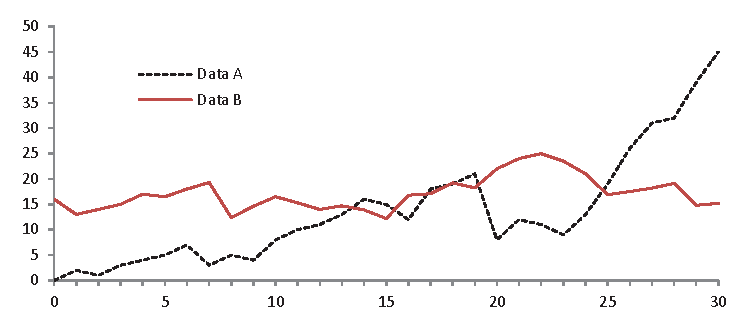
\includegraphics[width=\textwidth]{fig1.eps}
\caption{A figure caption is always placed below the illustration.
Please note that short captions are centered, while long ones are
justified by the macro package automatically.} \label{fig1}
\end{figure}

\begin{theorem}
This is a sample theorem. The run-in heading is set in bold, while
the following text appears in italics. Definitions, lemmas,
propositions, and corollaries are styled the same way.
\end{theorem}
%
% the environments 'definition', 'lemma', 'proposition', 'corollary',
% 'remark', and 'example' are defined in the LLNCS documentclass as well.
%
\begin{proof}
Proofs, examples, and remarks have the initial word in italics,
while the following text appears in normal font.
\end{proof}
For citations of references, we prefer the use of square brackets
and consecutive numbers. Citations using labels or the author/year
convention are also acceptable. The following bibliography provides
a sample reference list with entries for journal
articles~\cite{ref_article1}, an LNCS chapter~\cite{ref_lncs1}, a
book~\cite{ref_book1}, proceedings without editors~\cite{ref_proc1},
and a homepage~\cite{ref_url1}. Multiple citations are grouped
\cite{ref_article1,ref_lncs1,ref_book1},
\cite{ref_article1,ref_book1,ref_proc1,ref_url1}.
%
% ---- Bibliography ----
%
% BibTeX users should specify bibliography style 'splncs04'.
% References will then be sorted and formatted in the correct style.
%
% \bibliographystyle{splncs04}
% \bibliography{mybibliography}
%
%\begin{thebibliography}{8}
%\bibitem{ref_article1}
%Author, F.: Article title. Journal \textbf{2}(5), 99--110 (2016)
%
%\bibitem{ref_lncs1}
%Author, F., Author, S.: Title of a proceedings paper. In: Editor,
%F., Editor, S. (eds.) CONFERENCE 2016, LNCS, vol. 9999, pp. 1--13.
%Springer, Heidelberg (2016). \doi{10.10007/1234567890}
%
%\bibitem{ref_book1}
%Author, F., Author, S., Author, T.: Book title. 2nd edn. Publisher,
%Location (1999)
%
%\bibitem{ref_proc1}
%Author, A.-B.: Contribution title. In: 9th International Proceedings
%on Proceedings, pp. 1--2. Publisher, Location (2010)
%
%\bibitem{ref_url1}
%LNCS Homepage, \url{http://www.springer.com/lncs}. Last accessed 4
%Oct 2017
%\end{thebibliography}

\bibliographystyle{splncs04}
\bibliography{bibliography}

\end{document}
